\documentclass[11pt, oneside]{article}   	% use "amsart" instead of "article" for AMSLaTeX format
\usepackage{geometry}                		% See geometry.pdf to learn the layout options. There are lots.
\geometry{letterpaper}                   		% ... or a4paper or a5paper or ... 
%\geometry{landscape}                		% Activate for for rotated page geometry
%\usepackage[parfill]{parskip}    		% Activate to begin paragraphs with an empty line rather than an indent
\usepackage{graphicx}				% Use pdf, png, jpg, or eps� with pdflatex; use eps in DVI mode
								% TeX will automatically convert eps --> pdf in pdflatex		
\usepackage{amssymb}
\usepackage{amsmath}

\title{Approximation}
%\author{The Author}
%\section{}
% \subsection*{R code}
\date{}							% Activate to display a given date or no date

\graphicspath{{/Users/telliott_admin/Dropbox/Tex/png/}}
% \begin{center} 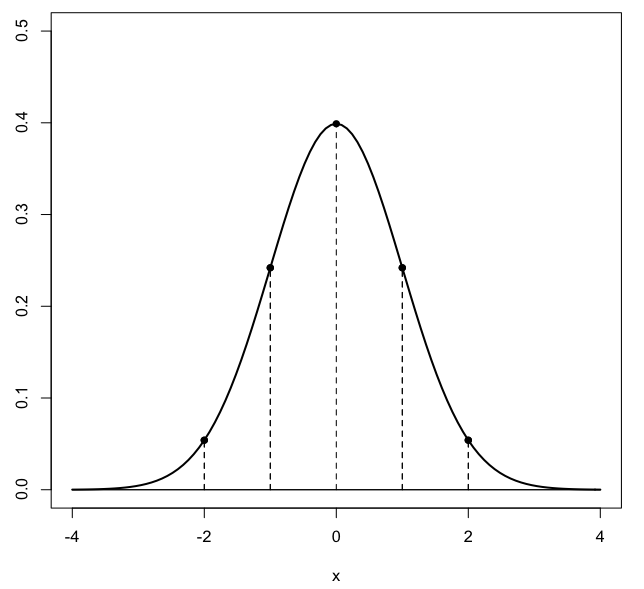
\includegraphics [scale=0.4] {gauss3.png} \end{center}

\begin{document}
\maketitle
\large
%\noindent
Some functions are easy to compute, while some are harder.  Any polynomial in $x$ is easy
\[ g(x) = a_0 + a_1x + a_2x^2 + a_3x^3 + \cdots \]

On the other hand, how would we compute $f(x) = e^x$?  It's not difficult for $x=0,1,2 \cdots$, but what about for $x=0.1$?  To begin with, let's try finding a polynomial function of $x$ that gives a value \emph{approximately equal} to that for the function $e^x$ in the neighborhood of the value $x=0$.

The very least we should require is that the value of $g(0) = f(0)$.
\[ f(x) = e^x  \approx f(0) = e^0 = 1 \]
For $g(x)$ to give the best answer
\[ g(0) = a_0 + a_1(0) + a_2(0)^2 + a_3(0)^3 + \cdots = a_0 \]
Evidently, if $g(0)=f(0)$ then $a_0$ must be equal to $1$.
\vspace{3mm}

The next step is to look for a linear approximation.  How much will $f(x)$ change from $f(0)$ for $x$ near $0$?  It will change by approximately $f'(0)$ times $x$.  So a better approximation is that
\[ f(x) = e^x \approx f(0) + f'(0)\ x  \]
If $f(x) = e^x$ then $f'(x)=e^x$ and $f'(0) = 1$ so
\[ f(x) \approx 1 + x  \]
For $g(x)$ to give the best answer
\[ g(x) = a_0 + a_1(x) = 1 + a_1(x) \]
Evidently, $a_1 = 1$ as well.  We want the slope of $g(x)$ to be equal to the slope of $f(x)$ at $x=0$.  
\vspace{3mm}

For a quadratic approximation, the secret is that the second derivatives must match.  $f''(x)=e^x$ at $x=0$ is still equal to $1$, but $g''(x)$ at $x=0$ is equal to $2a_2$.  So we have 
\[ f''(0) = 1 = g''(0) = 2a_2 \]
\[ a_2= \frac{1}{2} \]
\[ g(x) = 1 + x + \frac{1}{2}x^2 \]

Let's stop and see how accurate this is.  To ten places:
\[ e^{0.1} = 1.105170918 \]
Compare
\[ g(0.1) = 1 + 0.1 + \frac{1}{2}(0.1)^2 =  1 + 0.1 + 0.005000000 = 1.105 \]

To be even more accurate, we need the third derivatives to match.  Notice that when we differentiate $x^3$ twice we get first a factor of $3$ and then a factor of $2$, i.e. $3!$
\[ f'''(0) = 1 = g'''(0) = 3! \ a_3 \]
\[ a_3= \frac{1}{3!} \]
\[ g(x) = 1 + x + \frac{1}{2}x^2 + \frac{1}{3!}x^3 \]
Notice the pattern.  We have
\[ g(x) = \sum_{k=0}^{k = \infty} \ \frac{1}{k!}\  x^k \]
\[ = 1 +  \frac{x}{1!} + \frac{x^2}{2!} + \frac{x^3}{3!} + \cdots \]
When we use the whole (infinite) series, :), we have an \emph{exact} approximation
\[ e^0 = 1 + 1 + \frac{1}{2} + \frac{1}{6}  + \cdots \]
\[ e^x = 1 + x + \frac{x^2}{2} + \frac{x^3}{6}  + \cdots \]

In general, we have Taylor's Series as an approximation for $f(x)$ near $x=a$

\[ f(x) \approx f(a) + f'(a)\ (x-a) + \frac{f''(x)}{2!} (x-a)^2 + \frac{f'''(x)}{3!} (x-a)^3 + \cdots \]


\end{document}  